\documentclass[11pt,a4paper]{article}
\usepackage[utf8]{inputenc}
\usepackage{amsmath}
\usepackage{amsfonts}
\usepackage{amssymb}
\usepackage{graphicx}
\usepackage{geometry}
\usepackage[hidelinks]{hyperref}
\usepackage{booktabs}
\usepackage{float}
\usepackage{caption}
\usepackage{xcolor}
\usepackage{pdfpages}
\usepackage{circuitikz}
\usetikzlibrary{calc}

\definecolor{customblue}{RGB}{30, 69, 114} 
\definecolor{customgrey}{RGB}{133, 157, 181}


\hypersetup{
    colorlinks=true,
    linkcolor=customblue,
    filecolor=magenta,
    urlcolor=customblue,
}

\geometry{a4paper, margin=1in}

\graphicspath{{Images/}}

\author{Johnan Luca}

\date{\today}

\begin{document}

\begin{titlepage}
    \centering
    
    \vspace*{3cm}
    
    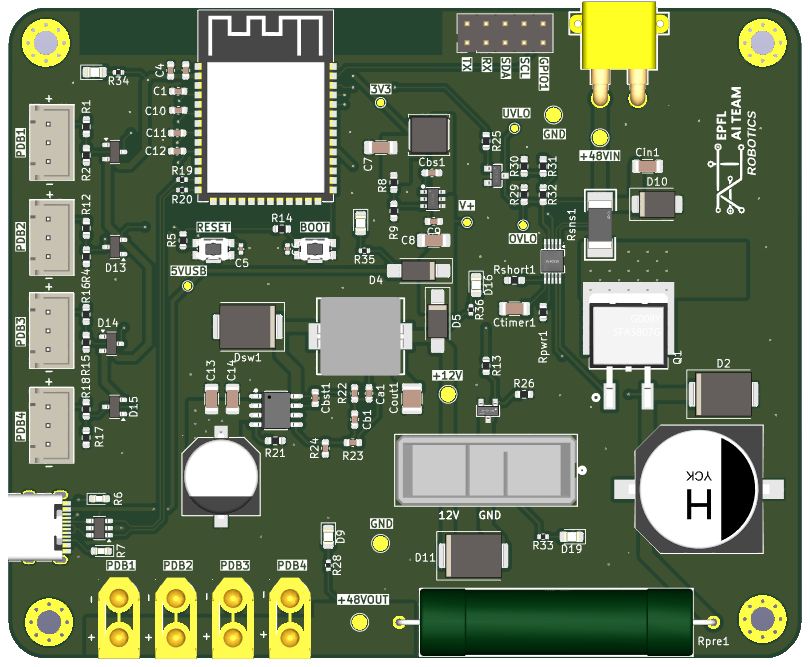
\includegraphics[width=8cm]{Images/GBL_ortho.png} 
    
    \vspace{2.5cm}
    
    % --- TITLE ---
    {\Huge Architecture Design, Sizing, and Vulnerability of the ``Good Boy Limiter''\par}
    
    \vspace{1.2cm}
    
    % --- DATE ---
    {\normalsize 13 October 2026 \par}
    {\small Revised 12 November 2026: system integration review (Section \ref{sec:review}) \par}
    {\small Revised 26 November 2026: pre-charge failure with the motors and GBL 2.0 changes (Section \ref{sec:gbl2}) \par}

    \vspace{1cm}

    {\large GBL version 1 \par}

     \vspace{1cm}
    
    % --- AUTHOR ---
    {\normalsize Johnan Luca \par} 
    {\normalsize BARK Project - AI Team-Robotics \par} 
    
    \vfill 
    
    % --- FOOTER ---
    {\footnotesize A practical documentation for understanding the GBL architecture and sizing of elements. \par}
    
\end{titlepage}

\tableofcontents
\newpage

\noindent\fcolorbox{red}{red!5}{\parbox{\dimexpr\linewidth-2\fboxsep-2\fboxrule\relax}{
\textbf{\color{red}CURRENT STATUS (26 November 2026) -- READ BEFORE POWERING THE ROBOT}

\smallskip
The GBL v1 mounted on the robot runs the \textbf{temporary emergency firmware} (\texttt{GBL\_Firmware\_emergency}), not the production firmware. With the twelve motor drivers connected the pre-charge cannot complete (Section \ref{sec:gbl2}), so this firmware closes the relay on a partially charged bus.

\smallskip
\textbf{The robot MUST NOT be powered at 48 V (12S or 13S) until the GBL 2.0 is installed.} At 6S the relay closes on a step of about 18 V and has survived repeated on/off cycles without any sign of degradation. At 12S the step would exceed 40 V: about five times the energy and more than twice the peak current through the contacts, with a real risk of welding them. A welded relay can no longer be opened by the GBL or by the emergency stop (which acts on the relay coil); only unplugging the battery disconnects the robot.

\smallskip
The emergency firmware is built for 6S only and aborts the pre-charge above 26.1 V. Do not modify this limit, do not select a 12S/13S pack, and do not remove the 100 k$\Omega$ UVLO resistor while this firmware is in use.
}}

\section{Abstract and System Overview}

The design of high-power DC distribution networks frequently encounters the engineering challenge of managing massive capacitive loads during the initial charging phase. The ``Good Boy Limiter'' (GBL) represents an hybrid power management and in-rush current control architecture specifically designed to address these challenges within a 48 V DC ecosystem.

The main problem addressed by the GBL architecture is the safe charge and continuous operation of a downstream load characterized by a really large input capacitance. Specifically, the system must interface with a bulk bus capacitance ($C_{tot}$) of 7920 $\mu$F, which is physically realized through a distributed $4 \times 6$ matrix of 330 $\mu$F electrolytic capacitors. Furthermore, the system is designed to support a substantial nominal operating current of 260 A, although it is currently constrained to a 120 A limit for safety reasons.

Attempting to directly connect a 48 V stiff voltage source to an uncharged 7920 $\mu$F capacitor bank results in an instantaneous "in-rush" current theoretically limited only by the Equivalent Series Resistance (ESR) of the capacitors and the parasitic inductance of the interconnecting cables. In practical terms, this transient current can easily exceed several thousands of amperes. Such catastrophic current spikes induce severe electromagnetic interference (EMI), trigger upstream power supply overcurrent protections, and instantly weld the contacts of mechanical relays due to localized plasma arcing.

To resolve these conflicting requirements, the GBL employs a mixed relay/solid-state architecture. A heavy-duty mechanical external relay (actuated via a 12 V coil) serves as the primary conduction path during nominal steady-state operation. In parallel, a highly controlled solid-state pre-charge circuit, orchestrated by the Texas Instruments LM5069-2 hot-swap controller and an STMicroelectronics STB15810 MOSFET, governs the initial energization phase.

This report provides an exhaustive analysis of the pre-charge dynamics, focusing on the mathematical sizing of the LM5069-2 control parameters. It critically examines the thermal paradigm shift achieved by the inclusion of a series limiting resistor, assesses the Safe Operating Area (SOA) of the selected MOSFET, and documents the role of the ESP32-S3 microcontroller in mitigating topological safety vulnerabilities.

\section{Power Architecture: Relay Versus Solid-State}

High-current DC power distribution systems inherently suffer from the physical limitations of their switching elements. The architectural decision to utilize a hybrid system in the Good Boy Limiter is grounded in fundamental power dissipation physics.

\subsection{The Limitations of Pure Solid-State Switching}
In a hypothetical pure solid-state architecture managing the full 260 A nominal current, the conduction losses would be to high. Even utilizing state-of-the-art power MOSFETs exhibiting an ultra-low drain-to-source on-resistance ($R_{DS(on)}$) of 1 m$\Omega$, the continuous power dissipation ($P_{loss}$) would be substantial. According to Joule's law:
\begin{equation}
P_{loss} = I^2 \times R_{DS(on)} = (260 \text{ A})^2 \times 0.001\ \Omega = 67.6 \text{ W}
\end{equation}
Dissipating 67.6 W of pure thermal energy on a printed circuit board (PCB) requires massive copper planes, extensive thermal via arrays, large extruded aluminum heatsinks, and mandatory active forced-air cooling. This increases volumetric footprint, acoustic noise, and overall system failure rates. 

\subsection{The Limitations of Pure Mechanical Switching}
Vice-versa, a purely mechanical relay architecture offers micro-ohm contact resistance, virtually eliminating steady-state thermal dissipation. However, mechanical relays are physically incapable of closing into an uncharged 7920 $\mu$F capacitive bus at 48 V. As the relay contacts physically approach one another during closure, the dielectric breakdown voltage of the microscopic air gap is exceeded. This initiates a high-energy plasma arc. The thousands of amperes of in-rush current flowing through this plasma instantly melt the contact plating, leading to contact welding and permanent failure of the relay.

\subsection{The Hybrid Resolution}
The GBL architecture resolves this dichotomy via a parallel power path topology:
\begin{itemize}
    \item \textbf{The Solid-State Pre-Charge Path:} Engaged first, this path utilizes a series-pass N-channel MOSFET (STMicroelectronics STB15810) and a 50 $\Omega$ wirewound power resistor (EWWR0010J50R0T9) to strictly limit the transient charging current. The capacitors are charged safely over a calculated time domain.
    \item \textbf{The Main Relay Path:} Engaged only when the ESP32-S3 microcontroller verifies that the bus voltage has reached the nominal source voltage. Because the voltage differential ($\Delta V$) across the relay contacts is near zero, the corresponding current during closure is zero. Closing the relay under this Zero-Voltage Switching (ZVS) entirely eliminates arcing, preserving contact longevity. Once the relay is closed, the solid-state path is disabled.
\end{itemize}

\section{Analysis and Sizing of the Pre-Charge Dynamics}

The pre-charge network is mathematically modeled as a first-order ideal RC circuit. The primary system parameters dictate a DC source voltage ($V_{IN}$) of 48 V, a total bus capacitance ($C_{tot}$) of 7920 $\mu$F, and a physical current-limiting series resistance ($R_{pre}$) of 50 $\Omega$.

\begin{figure}[H]
\centering

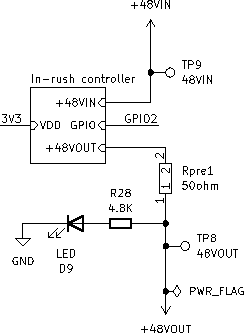
\includegraphics[width=0.35\textwidth]{Images/precharge.pdf}

\caption{Detail of the solid-state pre-charge topology. The 50 $\Omega$ resistor $R_{PRE1}$ dominates the branch impedance, physically limiting the maximum current to 0.96 A regardless of the state of the LM5069 controller.}
\end{figure}

\subsection{Peak In-Rush Current Constraint}
The theoretical peak current ($I_{peak}$) occurs instantaneously at $t=0$, assuming the capacitor bank is fully discharged ($V_C = 0\text{ V}$). The peak current is defined by Ohm's Law across the series resistor:
\begin{equation}
I_{peak} = \frac{V_{IN}}{R_{pre}} = \frac{48 \text{ V}}{50\ \Omega} = 0.96 \text{ A}
\end{equation}
By actively restricting the peak current to a mere 0.96 A, the GBL architecture completely eliminates the stress on the upstream 48 V power supply. The upstream source perceives the startup event as a negligible, highly controlled 46 W load rather than a multi-kilowatt short circuit.

\subsection{Time Constant and RC Charging Profile}
The exponential voltage charging profile of the capacitor bank is governed by the RC time constant ($\tau$), which dictates the temporal response of the circuit:
\begin{equation}
\tau = R_{pre1} \times C_{tot} = 50\ \Omega \times 0.00792 \text{ F} = 0.396 \text{ s}
\end{equation}
The bus voltage as a function of time, $V_C(t)$, is defined by the standard step-response differential equation solution:
\begin{equation}
V_C(t) = V_{IN} \left( 1 - e^{\frac{-t}{\tau}} \right) = 48 \left( 1 - e^{\frac{-t}{0.396}} \right)
\end{equation}
In standard engineering practice, a capacitor is considered functionally charged at $3\tau$ (95.0\% of $V_{IN}$) and fully charged at $5\tau$ (99.3\% of $V_{IN}$). 

We can calculate the exact time required to reach the 95\% threshold (45.6 V):
\begin{equation}
t_{95\%} = 3 \times \tau = 3 \times 0.396 \text{ s} = 1.188 \text{ s}
\end{equation}
Furthermore, the time required to reach the 99\% threshold (47.5 V):
\begin{equation}
t_{99\%} = 5 \times \tau = 5 \times 0.396 \text{ s} = 1.980 \text{ s}
\end{equation}
These timing calculations define the minimum operational window required before the ESP32-S3 firmware can safely command the main mechanical relay to close. Actuating the relay before 1.188 s would risk residual arcing due to a significant remaining voltage differential.

\subsection{Energy Transfer Thermodynamics}
The total energy transferred from the 48 V source to fully charge the capacitor bank is derived from the energy stored in the electric field of the capacitors:
\begin{equation}
E_{cap} = \frac{1}{2} C_{tot} V_{IN}^2 = \frac{1}{2} \times 0.00792 \text{ F} \times (48 \text{ V})^2 = 9.1238 \text{ J}
\end{equation}
A fundamental principle of thermodynamics in RC charging circuits dictates that an exactly equal amount of energy is dissipated as heat within the resistive elements of the charging path. Therefore, regardless of the charging speed, exactly 9.12 J of thermal energy is deposited into the 50 $\Omega$ wire-wound resistor during every startup sequence. This will be critically analyzed in Section \ref{sec:thermal}.

\section{In-Rush Controller (LM5069) Analysis and Sizing}

The Texas Instruments LM5069-2 operates as the gate driver and primary hardware safety controller for the solid-state pre-charge branch.

The following subsections detail the mathematical sizing of its internal thresholds.

\subsection{Undervoltage Lockout (UVLO) Sizing}
The UVLO pin ensures the controller only activates when the input bus is stable and possesses sufficient voltage to properly drive the downstream loads. The LM5069 possesses a precise internal comparator with an enable threshold of 2.5 V. To prevent rapid ON/OFF oscillation (chattering) when the input voltage fluctuates near the threshold, the IC utilizes an internal 21 $\mu$A current source to provide a programmable hysteresis. 

The GBL schematic defines a dedicated UVLO resistive divider utilizing $R_{31} = 143 \text{ k}\Omega$ as the top resistor and $R_{30} = 10 \text{ k}\Omega$ as the bottom resistor connected to ground.

The rising input threshold voltage ($V_{\text{UVLO\_RISE}}$) at which the controller enables the pre-charge sequence is calculated as:
\begin{equation}
V_{\text{UVLO\_RISE}} = V_{REF} \times \frac{R_{31} + R_{30}}{R_{30}} = 2.5 \text{ V} \times \frac{143 \text{ k}\Omega + 10 \text{ k}\Omega}{10 \text{ k}\Omega} = 38.25 \text{ V}
\end{equation}

Once the input voltage exceeds 38.25 V, the 21 $\mu$A internal current source activates and flows out of the UVLO pin, through the bottom resistor $R_{30}$, effectively raising the pin voltage. This creates the hysteresis voltage ($V_{\text{UVLO\_HYS}}$), which is dictated by the current source acting upon the top resistor $R_{31}$:
\begin{equation}
V_{\text{UVLO\_HYS}} = I_{HYS} \times R_{31} = 21 \text{ }\mu\text{A} \times 143 \text{ k}\Omega = 3.003 \text{ V}
\end{equation}

The falling threshold voltage ($V_{\text{UVLO\_FALL}}$), where the controller will abort the sequence due to a sagging input bus, is therefore:
\begin{equation}
V_{\text{UVLO\_FALL}} = V_{\text{UVLO\_RISE}} - V_{\text{UVLO\_HYS}} = 38.25 \text{ V} - 3.003 \text{ V} = 35.247 \text{ V}
\end{equation}
Therefore, the pre-charge sequence is hardware-locked until the input voltage is a steady 38.25 V, and it possesses a robust 3 V noise margin before shutting down at 35.24 V.

\subsection{Overvoltage Lockout (OVLO) Sizing}
Similarly, the OVLO pin protects the downstream systems from catastrophic input voltage surges, such as load-dump events or incorrect power supply connections. To maintain precise and independent control over the overvoltage threshold, the GBL schematic utilizes a separate, dedicated divider string: $R_{32} = 210 \text{ k}\Omega$ as the top resistor and $R_{29} = 10 \text{ k}\Omega$ as the bottom resistor.

The rising overvoltage cutoff threshold ($V_{\text{OVLO\_RISE}}$) is calculated using the same 2.5 V internal reference:
\begin{equation}
V_{\text{OVLO\_RISE}} = V_{REF} \times \frac{R_{32} + R_{29}}{R_{29}} = 2.5 \text{ V} \times \frac{210 \text{ k}\Omega + 10 \text{ k}\Omega}{10 \text{ k}\Omega} = 55.00 \text{ V}
\end{equation}

The OVLO pin also features a 21 $\mu$A hysteresis current source. The hysteresis voltage is:
\begin{equation}
V_{\text{OVLO\_HYS}} = I_{HYS} \times R_{32} = 21 \text{ }\mu\text{A} \times 210 \text{ k}\Omega = 4.410 \text{ V}
\end{equation}

The falling recovery threshold ($V_{\text{OVLO\_FALL}}$), where the system permits operation to resume after an overvoltage event clears, is:
\begin{equation}
V_{\text{OVLO\_FALL}} = V_{\text{OVLO\_RISE}} - V_{\text{OVLO\_HYS}} = 55.00 \text{ V} - 4.41 \text{ V} = 50.59 \text{ V}
\end{equation}

The hardware overvoltage cutoff is situated at 55.00 V. This provides adequate operational margin above the nominal 48 V state, while strictly protecting downstream components from transient degradation.

\begin{figure}[H]
\centering
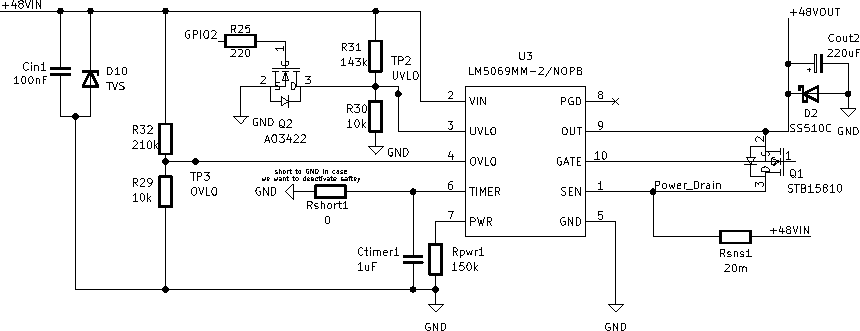
\includegraphics[width=0.7\textwidth]{Images/LM5069.pdf}
\caption{Schematic of the independent resistive dividers for the undervoltage ($R_{31}$, $R_{30}$) and overvoltage ($R_{32}$, $R_{29}$) thresholds. The use of two separate networks ensures clear and independent hysteresis for the operating windows at 38.25 V and 55.00 V.}
\end{figure}

\subsection{Hardware Current Limit (\texorpdfstring{$I_{LIM}$}{I\_LIM}) and $R_{sns1}$ Sizing}
The standard operational mode of the LM5069 relies on sensing the voltage drop across a precision shunt resistor ($R_{SENS1}$) placed directly between the \textbf{VIN} and \textbf{SENSE} pins. If the load current increases such that the voltage across the sense resistor reaches 55 mV, the LM5069 limits the current by dynamically adjusting the MOSFET gate voltage.

In the GBL design, a value for $R_{SENS1} = 20 \text{ m}\Omega$ is utilized. The absolute hardware current limit is established mathematically as:
\begin{equation}
I_{LIM} = \frac{V_{SNS(th)}}{R_{SENS1}} = \frac{55 \text{ mV}}{20 \text{ m}\Omega} = 2.75 \text{ A}
\end{equation}

\subsection{Power Limit Sizing (\texorpdfstring{$P_{FET(LIM)}$}{P\_FET(LIM)})}
To protect the external MOSFET from violating its Safe Operating Area (SOA) during linear mode regulation, the LM5069 allows the maximum allowable power dissipation of the FET to be programmed via the PWR pin. The LM5069 monitors the $V_{DS}$ of the MOSFET by comparing the SENSE pin and the OUT pin.

This limit is set using an external resistor ($R_{PWR1}$) connected to the PWR pin. The schematic indicates $R_{PWR1} = 150 \text{ k}\Omega$. 

The formula correlating the programmable power limit to the sense resistor and the PWR resistor is provided by Texas Instruments as:
\begin{equation}
P_{FET(LIM)} = \frac{R_{PWR1}}{1.25 \times 10^5 \times R_{SENS1}} = \frac{150,000\ \Omega}{1.25 \times 10^5 \times 0.020\ \Omega} = 60 \text{ W}
\end{equation}

The hardware is theoretically configured to throttle the MOSFET gate if it detects the MOSFET is dissipating more than 60 W of heat. However, the presence of the 50 $\Omega$ resistor ensures the MOSFET never dissipates anywhere near 60 W. This will be proven in Section \ref{sec:soa}.

\subsection{Fault Timer Duration (\texorpdfstring{$t_{FAULT}$}{t\_FAULT})}
The fault timeout allows the system to ride through brief, acceptable transient over-currents without nuisance tripping, but ensures the MOSFET is definitively shut down if a fault persists long enough to threaten the system. The timing is dictated by an external capacitor $C_{TIMER1} = 1 \text{ }\mu\text{F}$ connected to the TIMER pin.

The typical duration before a fault is declared and the gate is pulled low is defined by the equation:
\begin{equation}
t_{FAULT} = C_{TIMER1} \times \frac{v_{timer,typ}}{i_{timer,typ}} = 1 \times 10^{-6} \text{ F} \times 4.7 \times 10^4 = 0.047 \text{ s} = 47 \text{ ms}
\end{equation}

The specific LM5069-2 variant utilized in this design features an Auto-Retry mechanism. If the controller were to enter a current or power limit regulation state for longer than the 47 ms timer, the device would shut down the MOSFET, run through an extended internal cool-down cycle (dictated by the same capacitor), and then attempt to restart the process automatically. However, as established, the controller is physically prevented from ever entering the regulation state due to the 50 $\Omega$ resistor.

\section{Thermal Management and MOSFET Safe Operating Area (SOA)}
\label{sec:soa}

The defining architectural characteristic of the GBL pre-charge circuit is the intentional shifting of the massive thermal dissipation burden away from the semiconductor lattice of the STB15810 MOSFET and onto the robust, passive wirewound resistor.

\subsection{The STB15810 MOSFET in Deep Saturation}

In the Good Boy Limiter architecture, the presence of the 50 $\Omega$ resistor physically restricts the maximum current to 0.96 A. Because 0.96 A is vastly lower than the LM5069's 2.75 A current regulation threshold, the LM5069's internal high-side charge pump continues to pump unabated. It fully enhances the MOSFET gate, raising $V_{GS}$ to its maximum value (typically 10 V to 12 V above the source). This pushes the MOSFET completely out of the linear region and deep into the ohmic region (saturation).

The STB15810 is a heavily over-specified 100 V, 110 A device utilizing advanced STripFET™ F7 trench gate technology, boasting an ultra-low $R_{DS(on)}$ of 3.9 m$\Omega$ typical and 7 m$\Omega$ absolute maximum. 

Assuming the worst-case scenario at maximum operating junction temperature where $R_{DS(on)} = 7 \text{ m}\Omega$, the peak power dissipated by the MOSFET during the absolute highest current flow of the pre-charge phase (0.96 A at $t=0$) is simply calculated using Joule's law for a pure resistance:
\begin{equation}
P_{MOSFET(peak)} = I_{peak}^2 \times R_{DS(on)} = (0.96 \text{ A})^2 \times 0.007\ \Omega = 0.0064 \text{ W} = 6.4 \text{ mW}
\end{equation}

Dissipating a mere 6.4 mW means the STB15810 will experience absolutely zero measurable thermal rise above ambient temperature. The device remains entirely safe, utterly immune to the Spirito effect, and operates infinitely deep within the safest bounds of its DC SOA curve. From the perspective of thermal stress, the MOSFET acts as a perfect wire.

\section{Thermal Limitations: Analyzing the 50 $\Omega$ Power Resistor}
\label{sec:thermal}

Because the MOSFET acts as a near-perfect conductor, the 50 $\Omega$ wirewound resistor assumes basically 100\% of the thermal load during the pre-charge event. 

During the exact moment of turn-on ($t=0$), the capacitor bank acts as a short circuit, meaning the entire 48 V source is dropped across the resistor. The instantaneous peak power dissipation is:
\begin{equation}
P_{RESISTOR(peak)} = \frac{V_{IN}^2}{R_{pre}} = \frac{(48 \text{ V})^2}{50\ \Omega} = 46.08 \text{ W}
\end{equation}

The selected component, EWWR0010J50R0T9, is a wirewound power resistor rated for 10 W of continuous steady-state power. Operating a 10 W rated resistor at 46.08 W could appears as a design error; however, it is permissible because pre-charging is a highly transient pulse event, not a steady-state condition. 

As calculated in Equation (7), the total energy deposited into the resistor over the entire 1.5 to 2.0 second charging curve is strictly bounded to 9.12 J. Wirewound resistors are specifically constructed by winding a resistive alloy wire around a dense ceramic core. This ceramic core possesses a significant thermal mass. During a short 2-second pulse, the heating is largely adiabatic, the energy is absorbed directly into the thermal mass of the ceramic core, resulting in a moderate, entirely safe transient temperature rise. 

The critical operational limitation here is duty cycle: the system must not be commanded to repeatedly toggle the pre-charge sequence in rapid succession. Sufficient cool-down time (several seconds) must be enforced by the ESP32 software to allow the ceramic core to shed this thermal energy to the ambient environment.

\section{Control Logic, System Security, and the Software Timeout}

While the delegation of the current-limiting role to a passive 50 $\Omega$ resistor safely protects the MOSFET, it simultaneously creates a critical vulnerability within the hardware protection layers of the LM5069. This vulnerability necessitates the implementation of an active software safety supervisory system via the ESP32-S3 microcontroller.

\subsection{The ``Hardware Blind Spot'' during a Hard Short}
Consider a catastrophic operational scenario: a dead short circuit directly to ground exists on the 48 V output bus (e.g., a crushed cable or a failed downstream component) before the system is turned on.

When the ESP32 initiates the pre-charge sequence, the 50 $\Omega$ resistor performs its physical duty and limits the fault current:
\begin{equation}
I_{fault} = \frac{48 \text{ V}}{50\ \Omega + 0.020\ \Omega + 0.007\ \Omega} \approx 0.96 \text{ A}
\end{equation}

Because the fault current (0.96 A) is significantly lower than the LM5069 hardware current limit threshold (2.75 A), the LM5069 internal current comparator is never triggered. Furthermore, because the 50 $\Omega$ resistor is dropping nearly the entire 48 V, the voltage at the SENSE pin is roughly 0 V, and the $V_{DS}$ across the MOSFET is negligible (a few millivolts). Consequently, the power limit comparator ($P_{LIM} = 60 \text{ W}$) is also completely blind to the fault.

\textbf{The Catastrophic Result:} The LM5069 views the dead short circuit as a completely normal, healthy operating condition. The internal 47 ms fault timer ($C_{TIMER}$) never begins counting. The hardware safety system will remain engaged indefinitely, forcing the 10 W wirewound resistor to continuously dissipate 46.08 W. Within a matter of seconds, the resistor will violently exceed its thermal degradation limits, resulting in extreme overheating, outgassing, potential ignition of surrounding components, and ultimately an open-circuit failure.

\subsection{The ESP32-S3 Software Timeout Mitigation}
To permanently resolve this dangerous topological vulnerability, the ESP32-S3 microcontroller is tasked with monitoring the dynamic health of the pre-charge process via the dedicated Voltage Sensing Modules. 

\begin{figure}[H]
\centering
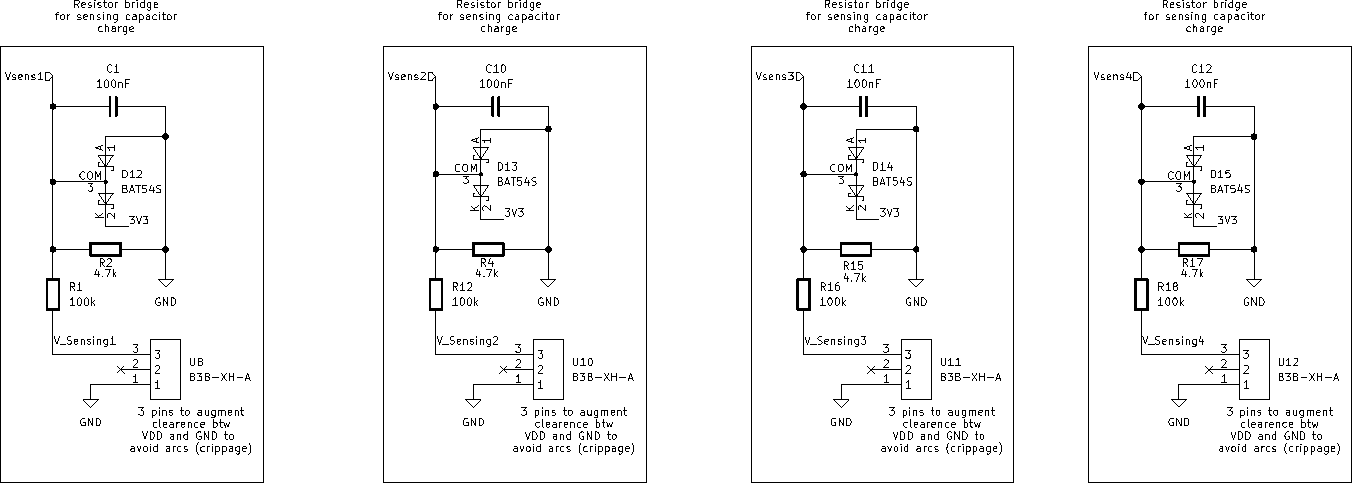
\includegraphics[width=0.7\textwidth]{Images/Sensing_modules.pdf}
\caption{Schematic diagram of the V\_Sensing modules used by the ESP32 to read the bus voltage. Note the resistor dividers connected to the BAT54S diodes, which are essential for protecting the microcontroller’s ADC inputs from transient overvoltages.}
\end{figure}

The ESP32 reads the intermediate bus voltage via a resistor divider string (100 k$\Omega$ top resistors $R_{1}$, $R_{12}$, $R_{16}$, $R_{18}$ over 4.7 k$\Omega$ bottom resistors, ratio 22.3). These inputs are aggressively protected by dual BAT54S Schottky clamping diodes, which prevent the microcontroller's sensitive ADC pins from exceeding the 3.3 V logic supply limit even during severe transients. 

The ESP32 firmware must be programmed to implement a strict, non-blocking state-machine timeout logic:
\begin{enumerate}
    \item \textbf{Initiation:} The ESP32 asserts the LM5069 EN/UVLO pin HIGH via a GPIO pin to begin the pre-charge sequence. Simultaneously, it initializes an internal hardware software timer ($t=0$).
    \item \textbf{Continuous Monitoring:} The ADC continuously samples the bus voltage ($V_{bus}$) at a high frequency.
    \item \textbf{Success Condition:} If $V_{bus}$ successfully exhibits the standard RC charging curve and exceeds 45 V (approximately $3\tau$) within a 1.5 to 2.0 second window, the pre-charge is deemed successful. The ESP32 then commands the main 12 V mechanical relay to close, routing the 260 A capability to the load. Once the relay confirms closure, the solid-state branch is deactivated. \textit{Revision note: the fixed 45 V threshold is only valid for an ideal 48 V source. The firmware does not use it: it detects the end of charge from the voltage slope; see Section \ref{sec:review_threshold}.}
    \item \textbf{Timeout Failure Condition (The Critical Mitigation):} If $V_{bus}$ fails to rise above a minimum safety threshold within 3.0 seconds (a ``Timeout of Security''), it is definitive proof of a downstream fault or short circuit absorbing the charge current. The ESP32 must immediately and unconditionally force the EN/UVLO pin LOW. This action forcefully shuts down the LM5069, halting the current flow and saving the 50 $\Omega$ resistor from thermal destruction.
\end{enumerate}
This software-defined safety boundary bridges the gap left by the hardware topology, ensuring full system resilience against all modes of failure.

\section{Auxiliary Power Supply: LM5013 DC-DC Converter}
\label{sec:LM5013}

To drive the heavy inductive coil of the main mechanical relay and provide logic-level power to the digital supervision systems, the GBL integrates a high-voltage auxiliary step-down (buck) converter based on the Texas Instruments LM5013DDAR. 

The LM5013 steps the primary 48 V distribution bus down to an intermediate 12 V rail. The converter is capable of handling inputs up to 100 V, providing massive immunity against 48 V bus ringing and transients. It operates utilizing a Constant On-Time (COT) architecture. COT control provides exceptional transient load response (essential when slamming a heavy relay coil) and entirely eliminates the need for complex external loop compensation networks (type II or type III compensators), simplifying the PCB layout.

\begin{figure}[H]
\centering
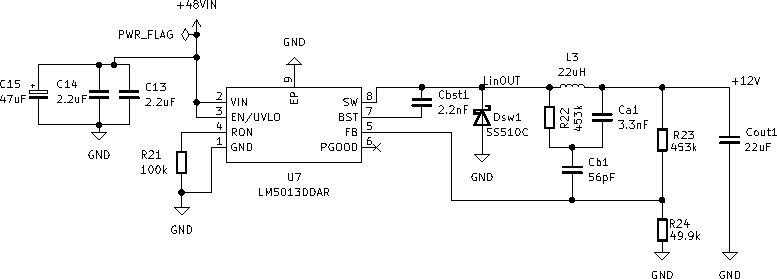
\includegraphics[width=0.8\textwidth]{Images/LM5013DDAR.pdf}
\caption{Topology of the LM5013 step-down converter. The main components are: the 22 $\mu$H inductor $L_{3}$, the bypass diode Dsw1 (SS510C), and the $R_{23}$/$R_{24}$ feedback network for precise regulation of the 12 V output.}
\end{figure}

\subsection{Feedback Sizing for the 12 V Rail}
The output voltage is programmed via a precision resistor divider feeding back into the FB pin. The highly precise internal bandgap reference voltage of the LM5013 is exactly $V_{REF} = 1.2 \text{ V}$. The schematic defines the top feedback resistor as $R_{FB1} (R_{23}) = 453 \text{ k}\Omega$ and the bottom resistor connected to ground as $R_{FB2} (R_{24}) = 49.9 \text{ k}\Omega$.

The nominal output voltage is mathematically derived as:
\begin{equation}
V_{OUT} = V_{REF} \times \left( 1 + \frac{R_{FB1}}{R_{FB2}} \right) = 1.2 \text{ V} \times \left( 1 + \frac{453 \text{ k}\Omega}{49.9 \text{ k}\Omega} \right)
\end{equation}

\begin{equation}
V_{OUT} = 1.2 \text{ V} \times \left( 1 + 9.078 \right) = 1.2 \text{ V} \times 10.078 = 12.09 \text{ V}
\end{equation}

\subsection{Core Buck Components and Filtering}
The power stage utilizes a low-DCR inductor $L_3 = 22 \text{ }\mu\text{H}$ and an SS510C Schottky freewheeling diode ($D_{SW1}$). The presence of the external Schottky diode is mandatory for this non-synchronous topology to provide a path for the inductor current during the MOSFET off-time. The Constant On-Time programming resistor is $R_{ON} (R_{21}) = 100 \text{ k}\Omega$, establishing the nominal switching frequency. 

Input voltage ripple and filtering are aggressively handled by dual low-ESR 2.2 $\mu$F ceramic capacitors ($C_{13}, C_{14}$) plus a larger 47 $\mu$F bulk capacitor ($C_{15}$). This network attenuates high-frequency switching noise, preventing the buck converter from injecting harmonic distortions back into the main 48 V distribution bus. A secondary step-down stage (utilizing the SY8120B buck converter) subsequently drops this intermediate 12 V to a highly regulated 3.3 V rail to power the ESP32-S3 microcontroller and its associated sensitive analog peripherals.

\section{Power Supply Logic and 3V3 Selector (SY8120B and Case Control)}

The ESP32-S3 and the analog logic arrays require a stable, low-noise 3.3V power rail. To ensure the microcontroller remains active and functional under multiple operating conditions, such as during initial programming via a PC (USB power), standalone operation from external logic batteries, or standard nominal operation connected to the main 48V bus, a specialized ``3V3 Selector'' architecture is implemented.

\begin{figure}[H]
\centering
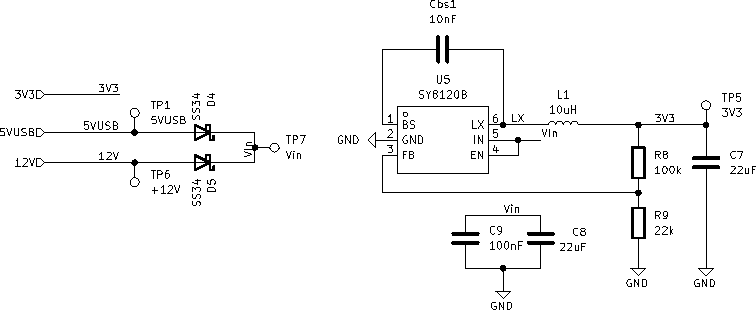
\includegraphics[width=0.8\textwidth]{Images/3V3.pdf}
\caption{Schematic diagram of the “3V3 Selector” module based on the SY8120B synchronous buck converter. Note the OR-gate diode configurations (D4 and D5) for transparent switching between the USB power supply and the 12V bus, and the R10/R11 feedback divider for precise regulation to 3.3V.}
\end{figure}

\subsection{Power Source OR-ing Network and Operational Scenarios}

The input to the 3.3V regulation stage ($V_{in}$) is sourced dynamically via a passive diode OR-ing network. This network prevents reverse-current back-feeding and allows the system to autonomously draw power from the most viable source without logic interruption. The system relies on two SS34 Schottky diodes (D4 and D5) which feature a low forward voltage drop ($V_f \approx 0.4$V at nominal logic currents).The architecture supports three distinct operational scenarios:

\begin{itemize}
\item \textbf{Case 1: PC Configuration Only (No Main Battery Connected).} \\
When the GBL is completely disconnected from the 48V high-voltage bus (no XT30 battery connected) and plugged into a host PC via the USB-C connector, the cable supplies $+5\text{V}_{USB}$. Diode D4 becomes forward-biased. The internal node $V_{in}$ reaches approximately $4.6\text{V}$ ($5\text{V} - V_{f(D4)}$). Because the SY8120B regulator has a minimum operational input threshold of 4.0V, it successfully activates, generating the 3.3V rail. This allows the ESP32 to be programmed, flashed, or debugged safely on a workbench without exposing the user to high-voltage hazards.

\item \textbf{Case 2: Main Battery / 48V Bus Nominally Connected.} \\
During standard operation, the main power source (e.g., a 48V battery pack) is connected to the XT30 connectors (CN1). The upstream LM5013 buck converter actively steps the 48V down to the intermediate $+12\text{V}$ rail. This 12V potential reaches the anode of diode D5. D5 becomes forward-biased, pulling the $V_{in}$ node to approximately $11.6\text{V}$ ($12\text{V} - V_{f(D5)}$). The SY8120B easily accepts this input (rated up to 18V maximum) and drops it to 3.3V. 

\item \textbf{Case 3: Both Main Battery and PC USB Connected.} \\
This is the most critical cross-power scenario. If a user connects the USB-C cable for telemetry while the 48V bus is fully live, the OR-ing network automatically resolves the power conflict. The anode of D5 sits at $+12\text{V}$, while the anode of D4 sits at $+5\text{V}_{USB}$. Because the cathodes of both diodes are tied together at the $V_{in}$ node, D5 will strongly conduct and pull the $V_{in}$ node up to $11.6\text{V}$. Consequently, the $+11.6\text{V}$ at the cathode of D4 is significantly higher than the $+5\text{V}$ at its anode. Diode D4 becomes heavily reverse-biased and stops conducting completely. \\ 
\textbf{Result:} The logic array draws zero power from the host PC's USB port, protecting the laptop's motherboard and ensuring the ESP32 is powered exclusively by the main battery line, while keeping the communication lines active for interfacing the MCU.

\end{itemize}

\subsection{SY8120B Synchronous Buck Converter Sizing}

Unlike the LM5013, the SY8120B is a \textit{synchronous} buck converter. It integrates both the high-side and low-side switching MOSFETs internally. These internal switches boast very low $R_{DS(on)}$ characteristics (145 m$\Omega$ top / 135 m$\Omega$ bottom), minimizing conduction losses and \textbf{entirely eliminating the need for an external Schottky freewheeling diode}.

The output voltage is programmed by the external resistor divider connected to the feedback (FB) pin. The internal bandgap reference voltage of the SY8120B is $V_{REF} = 0.6$V.Utilizing the designated top resistor $R_{10} = 100$ k$\Omega$ and the bottom resistor $R_{11} = 22$ k$\Omega$, the nominal output voltage is derived using the standard feedback formula:

\begin{equation}
V_{OUT} = V_{REF} \times \left( 1 + \frac{R_{10}}{R_{11}} \right) = 0.6\text{ V} \times \left( 1 + \frac{100\text{ k}\Omega}{22\text{ k}\Omega} \right)= 3.327\text{ V} 
\end{equation}


The calculated 3.327V output provides a regulated logic-level rail for the ESP32-S3. An external pull-up resistor $R_8 = 100$ k$\Omega$ connects the EN (Enable) pin directly to the input voltage node ($V_{in}$), ensuring the regulator automatically initiates switching the millisecond a valid power source (USB or Battery) is applied via the OR-ing networkr.
\section{Main Relay Actuation and Control Circuit}
The primary high-current conduction path of the GBL architecture relies on an external heavy-duty mechanical relay connected via U2 (TE Connectivity 1-178136-3). To interface the 3.3 V logic domain of the ESP32-S3 with the 12 V DC requirement of the relay coil, a dedicated low-side switching circuit is implemented on the PCB.

\subsection{Low-Side Switching Topology}
The relay coil is permanently tied to the +12 V auxiliary power rail at pin 3 of connector U2. The ground return path (pin 2) is dynamically controlled by an N-channel logic-level MOSFET, Q4 (AO3400A).

When the microcontroller asserts the \texttt{GPIO38} signal HIGH (3.3 V), Q4 enters conduction, pulling pin 2 to ground and energizing the relay coil. A 220 $\Omega$ series gate resistor (R13) limits the instantaneous transient current required to charge the MOSFET gate capacitance, protecting the ESP32 GPIO pin from overcurrent spikes. Furthermore, a 10 k$\Omega$ pull-down resistor (R26) ensures the gate is firmly held at 0 V during system boot or whenever the GPIO pin is in a high-impedance (floating) state, preventing unintended and dangerous relay activation.

\subsection{Inductive Transient Protection}
Due to the highly inductive nature of the relay coil, abruptly interrupting the coil current generates a massive reverse-voltage spike (back-EMF) as the internal magnetic field collapses. To protect the AO3400A MOSFET from exceeding its drain-to-source breakdown voltage, a Schottky flyback diode, D11 (SS510C), is placed in anti-parallel with the coil terminals (cathode connected to +12 V, anode to the MOSFET drain). This topology provides a safe, low-impedance freewheeling path to dissipate the inductive energy safely upon shutdown.

\subsection{Design Anomaly: LED Indicator Inversion and Parasitic Draw}
\textbf{Hardware Warning:} An architectural anomaly exists within the visual status signaling sub-circuit associated with the relay. The LED D19 and its current-limiting resistor R33 (1 k$\Omega$) are connected directly between the MOSFET drain (relay pin 2) and ground.

This topology results in an inverted logic state and an unintended continuous parasitic current draw:
\begin{itemize}
    \item \textbf{Relay OFF State (Q4 Open):} The +12 V potential traverses the relay coil, passing out of pin 2, through R33 and D19, to ground. This actively illuminates the LED when the relay is \textit{inactive}. Additionally, this establishes a continuous parasitic current of approximately 10 to 12 mA through the relay coil. While this current is insufficient to mechanically actuate the heavy relay contacts, it results in unnecessary thermal dissipation within the coil and constant power consumption from the 12 V rail.
    \item \textbf{Relay ON State (Q4 Closed):} The MOSFET pulls the drain to 0 V, eliminating the potential difference across the LED branch. As a result, the LED turns \textit{off} when the relay is successfully engaged, acting inversely to standard visual indication practices.
\end{itemize}

\textbf{Mitigation Strategy:} For future PCB revisions, the LED branch should be relocated to the logic side (driven directly by \texttt{GPIO38} to ground) or placed strictly in parallel with the coil. For the current hardware iteration, if the 12 mA parasitic draw is deemed unacceptable for battery operation, it is recommended to physically desolder and remove R33 from the PCB. This will open the parasitic circuit loop, accepting the loss of visual status indication in favor of strict electrical efficiency.

\section{LEDs}
\subsection{LED's Resistors Sizing}
To light an LED from a power rail, you simply place the LED in series with a current-limiting resistor across the rail and ground. You must calculate the correct resistance ($R$) using Ohm's Law for preventing the LED to burn out:
\begin{equation}
    R = \frac{V_{rail} - V_{f}}{I_{f}}
\end{equation}
\begin{itemize}
    \item $V_{rail}$: The voltage of your power rail (e.g., 3.3V, 5V, 12V).
    \item $V_{f}$: The Forward Voltage of the LED (typically 1.8V for Red, 3.2V for Blue/White).
    \item $I_{f}$: The Forward Current you want (typically 2mA to 20mA).
\end{itemize}

\subsection{GBL's LEDs Color Code}
\begin{itemize}
    \item \textbf{RED}: +48V Pre-charge power rail is ON
    \item \textbf{YELLOW}: +3V3 power rail is ON
    \item \textbf{GREEN}: Relay is closed
    \item \textbf{BLUE}: +5USB power rail is ON
    \item \textbf{ORANGE}: +12V rail is ON
\end{itemize}

\section{System Integration Review: Battery Operation (Revision of 12 November 2026)}
\label{sec:review}

The previous sections size the GBL against an ideal, fixed 48 V source. This section records what changes when the board is integrated in the robot (BYTE power scheme: battery, 100 A contactor, bus bars, four PDBs, twelve GIM8108-8 actuators with GDS68 drivers) and powered from LiPo batteries. Values marked \textit{to verify} are estimates or assumptions that have not been measured yet.

\subsection{Real Operating Voltage Window}

The robot is powered either by one 6S LiPo (bring-up) or by two identical 6S LiPo packs in series (12S). A battery is not a fixed 48 V source:

\begin{table}[H]
\centering
\begin{tabular}{lccc}
\toprule
Condition & Per cell & 6S & 12S \\
\midrule
Fully charged & 4.20 V & 25.2 V & 50.4 V \\
Nominal & 3.70 V & 22.2 V & 44.4 V \\
Recommended stop under load & 3.50 V & 21.0 V & 42.0 V \\
Absolute minimum & 3.20 V & 19.2 V & 38.4 V \\
\bottomrule
\end{tabular}
\caption{Battery voltage window that the GBL must handle.}
\end{table}

Recomputing the pre-charge figures of Section 3 at the worst case of 50.4 V:
\begin{align}
I_{peak} &= \frac{50.4 \text{ V}}{50\ \Omega} = 1.01 \text{ A} \\
P_{RESISTOR(peak)} &= \frac{(50.4 \text{ V})^2}{50\ \Omega} = 50.8 \text{ W} \\
E_{cap} &= \frac{1}{2} \times 0.00792 \text{ F} \times (50.4 \text{ V})^2 = 10.06 \text{ J}
\end{align}
The peak current remains far below the 2.75 A hardware limit and the pulse energy grows by only 10\%, so the conclusions of Sections \ref{sec:soa} and \ref{sec:thermal} still hold. The time constant (0.396 s) does not depend on the voltage.

The lockout thresholds map onto the 12S window as follows:
\begin{itemize}
    \item \textbf{UVLO (38.25 V rising, 35.25 V falling):} 38.25 V corresponds to 3.19 V per cell. The pre-charge cannot start on a depleted 12S pack, which is the desired behaviour.
    \item \textbf{OVLO (55.00 V rising, 50.59 V falling):} the margin above a full pack is 4.6 V. The GDS68 drivers accept up to 56 V, so the OVLO sits just below the driver limit. Note that the OVLO only gates the solid-state branch: once the relay is closed, a regenerative braking surge is not disconnected by the GBL. Note also that the recovery threshold (50.59 V) is only 0.19 V above a full pack (50.4 V).
\end{itemize}

\subsection{Temporary 6S Modification of the UVLO Divider}
\label{sec:review_uvlo}

To operate from a single 6S pack, a 100 k$\Omega$ resistor is currently soldered between UVLO and +48VIN, in parallel with the 143 k$\Omega$ top resistor:
\begin{equation}
R_{top} = \frac{143 \text{ k}\Omega \times 100 \text{ k}\Omega}{143 \text{ k}\Omega + 100 \text{ k}\Omega} = 58.85 \text{ k}\Omega
\end{equation}
\begin{align}
V_{\text{UVLO\_RISE}} &= 2.5 \text{ V} \times \frac{58.85 \text{ k}\Omega + 10 \text{ k}\Omega}{10 \text{ k}\Omega} = 17.21 \text{ V} \\
V_{\text{UVLO\_HYS}} &= 21\ \mu\text{A} \times 58.85 \text{ k}\Omega = 1.24 \text{ V}
\end{align}
The falling threshold is therefore 15.98 V.

\begin{itemize}
    \item \textbf{No hardware battery protection on 6S:} 15.98 V is 2.66 V per cell, well below the safe minimum of a LiPo. While the modification is fitted, over-discharge protection comes only from the firmware, which opens the line below 18 V (3.0 V per cell under load), and from external cell alarms.
    \item \textbf{The resistor may stay in place for 12S operation.} With it fitted, the UVLO pin rises to $50.4 \text{ V} \times 10 / 68.85 = 7.3$ V instead of 3.3 V, far below the 100 V absolute maximum rating of the UVLO pin (LM5069 datasheet, Section 7.1). The only effect is that the hardware 38.25 V lockout is lost. This lockout is redundant with the firmware, which refuses a pre-charge that settles below 3.2 V per cell (38.4 V) and opens the line below 3.0 V per cell (36 V). Removing the resistor restores the hardware backup but is not required. In both cases the 12S battery must be selected in the firmware configuration (menuconfig) and the board reflashed; no code change is needed.
\end{itemize}

\subsection{Voltage Sensing Range and PDB Topology}
\label{sec:review_vsense}

On the PDB (PDBueno\_pro) the two XT90 inputs are in series: the upper one sits between +44V4 and the net 22V2, the lower one between 22V2 and GND. The V\_Sensing connector measures the net 22V2 against GND. The bulk capacitors are all connected between +44V4 and GND.

With a single supply feeding the lower XT90 and the upper XT90 bridged (the present wiring, and the only practical one when the two packs are joined in series at the battery), the net 22V2 is the full bus voltage. The V\_Sensing input therefore sees up to 50.4 V on 12S, not half of it.

The sensing divider is 100 k$\Omega$ / 4.7 k$\Omega$ (ratio 22.3) with a 100 nF filter and BAT54S clamps. With the 12 dB ADC attenuation used by the firmware, the full scale is about 69 V, so the range covers 6S, 12S and 13S packs without any hardware change. The firmware converts with eFuse calibration, averages 16 samples per reading and applies a per-channel gain correction.

\begin{table}[H]
\centering
\begin{tabular}{lcc}
\toprule
Battery state & Bus voltage & ADC pin voltage \\
\midrule
6S at 3.3 V per cell & 19.8 V & 0.89 V \\
6S full & 25.2 V & 1.13 V \\
12S at 3.3 V per cell & 39.6 V & 1.78 V \\
12S full & 50.4 V & 2.26 V \\
OVLO threshold & 55.0 V & 2.47 V \\
\bottomrule
\end{tabular}
\caption{ADC pin voltage with the 100 k$\Omega$ / 4.7 k$\Omega$ sensing divider. All operating points are inside the linear region of the ESP32 ADC.}
\end{table}

\subsection{Relay Closing Criterion}
\label{sec:review_threshold}

The success condition described in Section 7.2 (bus above 45 V) is not valid with a battery: with a full 12S pack 45 V is only 89\% of the source, and with a pack below 45 V it is never met. The firmware (GBL\_Firmware, \texttt{gbl\_power.c}) does not use it. Because the GBL v1 does not measure the battery voltage, the end of charge is detected from the voltage slope:
\begin{enumerate}
    \item \textbf{Sampling:} all enabled PDB channels are read every 20 ms.
    \item \textbf{Short-circuit check:} abort if any PDB is still below 5 V after 300 ms.
    \item \textbf{Consistency check:} abort if the PDB voltages differ by more than 0.15 V per cell (0.9 V on 6S, 1.8 V on 12S).
    \item \textbf{Plateau detection:} the charge is complete when no PDB rises by more than 0.1 V in 200 ms.
    \item \textbf{Plausibility:} the plateau must lie between 3.2 V and 4.35 V per cell (19.2 V to 26.1 V on 6S, 38.4 V to 52.2 V on 12S), otherwise abort.
    \item \textbf{Timeout:} abort after 3.0 s. An independent watchdog switches Q1 off after 3.5 s, and a 10 s cooldown is enforced between two pre-charges.
    \item \textbf{Closure:} relay closed, then Q1 off after 100 ms.
\end{enumerate}
While the line is on, the firmware opens it if the bus stays below 3.0 V per cell for 100 ms. The shutdown is controlled: Q1 is switched on in parallel, the relay is opened and Q1 is switched off 200 ms later.

\textbf{Residual weakness:} the plausibility window is as wide as the whole battery range, so it does not bound the voltage difference across the contacts at closure. A fully charged 12S pack (50.4 V) whose bus settles at 39 V because of a static load (Section \ref{sec:review_load}) passes every check, and the relay then closes on an 11 V difference. The resulting current step is roughly $\Delta V / R_{loop}$, where $R_{loop}$ is the sum of battery internal resistance, wiring and capacitor ESR (a few tens of milliohms, \textit{to verify}), i.e. hundreds of amperes. Until the battery voltage is measured on the board, this must be excluded by measurement: the ``charged'' line of the firmware log gives the plateau of each PDB, to be compared with the battery voltage read with a multimeter.

\subsection{Static Load on the Bus During Pre-Charge}
\label{sec:review_load}

The RC model of Section 3 assumes that the bus is a pure capacitance. In the robot, several loads are connected downstream of the relay and draw current through the 50 $\Omega$ resistor during pre-charge. The bus then settles at
\begin{equation}
V_{plateau} = V_{BATT} - R_{pre} \times I_{load}
\end{equation}
Known and expected contributions at 50.4 V:
\begin{itemize}
    \item \textbf{PDB bleed resistors:} four 47 k$\Omega$ resistors in parallel per PDB (11.75 k$\Omega$), i.e. 4.3 mA per board and 17.2 mA for four boards.
    \item \textbf{GBL output LED (D9, $R_{28}$ = 4.8 k$\Omega$):} about 10 mA.
    \item \textbf{Twelve motor drivers at idle and the 12 V buck of the Jetson:} not measured yet (\textit{to verify}). These are expected to dominate.
\end{itemize}

\begin{table}[H]
\centering
\begin{tabular}{cccc}
\toprule
$I_{load}$ & Drop on $R_{pre}$ & Plateau at 50.4 V & Power in $R_{pre}$ \\
\midrule
27 mA (bleed + LED) & 1.4 V & 49.0 V & 0.04 W \\
100 mA & 5.0 V & 45.4 V & 0.5 W \\
300 mA & 15.0 V & 35.4 V & 4.5 W \\
500 mA & 25.0 V & 25.4 V & 12.5 W \\
\bottomrule
\end{tabular}
\caption{Effect of a static load on the pre-charge plateau. Reaching 95\% of the battery voltage requires less than about 50 mA of total load.}
\end{table}

Consequences and actions:
\begin{itemize}
    \item Even with no other load, the bus never reaches the battery voltage exactly (about 1.4 V below). The closing criterion must be a plateau, not equality with the source.
    \item Converters behave as constant-power loads: as the bus voltage drops they draw more current, so the bus can latch at a low voltage and the pre-charge never completes.
    \item \textbf{Measurement required:} compare the plateau voltage reported in the firmware log at the end of pre-charge, with all loads connected, with the battery voltage. This single measurement decides whether $R_{pre}$ must be changed.
    \item \textbf{If the plateau is too low:} keep the Jetson buck disabled until the relay is closed, and reduce $R_{pre}$. With the present $R_{SENS1}$ the lower bound is $50.4 \text{ V} / 2.75 \text{ A} = 18.3\ \Omega$; a 22 $\Omega$ resistor gives a 2.3 A peak, a 0.17 s time constant and the same 10 J pulse energy, with a 115 W peak that must be checked against the pulse rating of the resistor.
    \item \textbf{$R_{28}$ dissipation:} with the bus at 50.4 V, $R_{28}$ dissipates about 0.49 W continuously. Its package power rating must be checked (\textit{to verify}).
\end{itemize}

\subsection{System-Level Protection}

\begin{itemize}
    \item \textbf{Actual current rating:} the main path is limited by the installed contactor (EV-type, 100 A continuous, 1000 V DC) and not by the 260 A / 120 A figures quoted in Section 1. The expected average current is 10 A to 30 A, with short peaks above 100 A (\textit{to verify} with CAN logs).
    \item \textbf{Main fuse (missing in v1):} a bolt-down fuse rated for at least 58 V DC must be placed on the positive battery lead. Recommended: Littelfuse MIDI 70V HP or MEGA 70V HP, 100 A, with 2500 A interrupting rating at 70 V DC. Fuses rated 32 V, and 58 V types with only 1000 A interrupting rating, are not suitable for a 12S LiPo, whose short-circuit current is estimated above 1500 A.
    \item \textbf{GBL supply fuse:} the 14 AWG feed to V\_BATT is taken upstream of the relay and needs its own small in-line fuse (5 A).
    \item \textbf{Capacitor voltage rating:} the PDB capacitors (VZH331M2A, 330 $\mu$F) appear to be 100 V parts from the part code; $C_{out2}$ on the GBL must be rated at least 63 V (\textit{to verify}).
\end{itemize}

\subsection{Operating Two 6S Packs in Series}

The packs have no internal protection (the Spektrum Smart electronics only log data). The following rules apply:
\begin{itemize}
    \item identical packs, with similar age and cycle count, both fully charged before being connected;
    \item the series link is opened for charging and each pack is balance-charged separately as a 6S pack;
    \item no power load is taken from the mid-point between the packs (a high-impedance voltage measurement is acceptable);
    \item one cell alarm per pack on the balance connector, because the total voltage does not reveal a single weak cell. The balance connector of the upper pack sits between 25 V and 50 V above system ground and must not share a non-isolated measurement circuit with the lower pack;
    \item when changing from 6S to 12S: select the 12S battery in the firmware configuration (menuconfig) and reflash. The 100 k$\Omega$ UVLO resistor may stay in place (Section \ref{sec:review_uvlo}).
\end{itemize}

\subsection{Proposed Electronic 6S/12S Selection (Next Revision)}
\label{sec:review_autodetect}

In v1 the battery type is set in two places: a hand-soldered resistor for the hardware UVLO and a compile-time option for the firmware. Both require access to the board. The next revision should select the battery without any manual operation.

\subsubsection{Battery Voltage Measurement}
A fifth sensing channel is added on +48VIN, upstream of Q1 and of the relay, identical to the PDB channels: 100 k$\Omega$ / 4.7 k$\Omega$ divider, 100 nF filter and BAT54S clamp, on a free ADC1 pin of the ESP32-S3 (pin to be chosen against the pinout). The divider draws about 0.5 mA from a full 12S pack.

\subsubsection{Automatic Detection}
The resting voltage windows of the two packs do not overlap (a full 6S pack reaches 25.2 V, an empty 12S pack starts at 36 V), so the measured input voltage identifies the battery:

\begin{table}[H]
\centering
\begin{tabular}{lc}
\toprule
Measured +48VIN at rest & Decision \\
\midrule
18.0 V to 26.1 V & 6S \\
36.0 V to 52.2 V & 12S \\
anything else & fault, the line is not started \\
\bottomrule
\end{tabular}
\caption{Battery identification from the input voltage. A 13S pack (39.0 V to 56.6 V) overlaps the 12S window and cannot be told apart automatically; it would remain an explicit configuration.}
\end{table}

Firmware sequence:
\begin{enumerate}
    \item \textbf{Boot:} outputs in their safe state (Q1 disabled, relay open, UVLO range at its default).
    \item \textbf{Measure:} +48VIN is averaged over about 100 ms with the line off.
    \item \textbf{Classify:} the cell count is chosen from the table above. It becomes a run-time variable; every per-cell threshold of the firmware (pre-charge window, PDB spread, undervoltage while on) is derived from it, as is done today from the compile-time option.
    \item \textbf{Latch:} the decision is taken only while the line is off and is kept until the next power-off, so a voltage sag under load can never change it.
    \item \textbf{Close check:} at the end of the pre-charge the relay is closed only if the difference between +48VIN and the lowest PDB voltage is below a limit (for example 2 V). This removes the residual weakness described in Section \ref{sec:review_threshold}.
\end{enumerate}

\subsubsection{Hardware UVLO Threshold}
Two implementations are possible.

\textbf{Option A, fixed low threshold (recommended).} The UVLO divider is sized once for the 6S pack and the per-battery limits are left to the firmware, which already enforces them. With $R_{31} = 143 \text{ k}\Omega$ and $R_{30} = 23.2 \text{ k}\Omega$:
\begin{equation}
V_{\text{UVLO\_RISE}} = 2.5 \text{ V} \times \frac{143 \text{ k}\Omega + 23.2 \text{ k}\Omega}{23.2 \text{ k}\Omega} = 17.9 \text{ V}, \qquad V_{\text{UVLO\_FALL}} = 17.9 \text{ V} - 3.0 \text{ V} = 14.9 \text{ V}
\end{equation}
No additional component is needed. This is electrically equivalent to v1 with the 100 k$\Omega$ resistor fitted.

\textbf{Option B, threshold switched by a GPIO.} If the 38 V hardware lockout must be kept for 12S, a second bottom resistor is switched in parallel with $R_{30}$ by a small N-channel MOSFET (the AO3422 already used for Q2 is suitable), as shown in Figure \ref{fig:uvlo_sel}.

\begin{figure}[H]
\centering
\begin{circuitikz}[european resistors, font=\small]
    % UVLO divider
    \draw (0,6.5) node[above]{+48VIN} to[short, o-] (0,6)
          to[R, l_={$R_{31}$ 143 k$\Omega$}] (0,3.5) coordinate (uvlo);
    \draw (uvlo) to[short, *-o] (-2.2,3.5) node[left]{UVLO (LM5069)};
    \draw (uvlo) to[R, l_={$R_{30}$ 23.2 k$\Omega$}] (0,0.8) node[ground]{};
    % switched bottom resistor
    \draw (uvlo) -- (3,3.5) to[R, l_={$R_{sel}$ 17.4 k$\Omega$}] (3,1.9);
    \draw (3,1.9) node[nmos, anchor=D, xscale=-1] (q5) {};
    \node[left] at ($(q5.D)!0.5!(q5.S) + (-0.1,0)$) {Q5 AO3422};
    \draw (q5.S) node[ground]{};
    % gate: pull-up to 3V3 and GPIO
    \draw (q5.G) -- ++(1.8,0) coordinate (g);
    \draw (g) to[R, *-, l_={100 k$\Omega$}] ++(0,2.4) node[vcc]{3V3};
    \draw (g) to[short, -o] ++(1.6,0) node[right]{GPIO (range)};
\end{circuitikz}
\caption{Proposed GPIO-switched UVLO threshold (Option B). With Q5 off the bottom resistance is $R_{30}$ alone (6S range, 17.9 V rising); with Q5 on, $R_{sel}$ is added in parallel (12S range, 38.5 V rising). The 100 k$\Omega$ pull-up keeps Q5 on, i.e. the safe 12S range, while the ESP32 is in reset or booting.}
\label{fig:uvlo_sel}
\end{figure}

\begin{itemize}
    \item \textbf{Q5 off (GPIO driven low): 6S range.} Bottom resistance 23.2 k$\Omega$, threshold 17.9 V rising, 14.9 V falling.
    \item \textbf{Q5 on (GPIO high or floating): 12S range.} Bottom resistance $23.2 \text{ k}\Omega \parallel 17.4 \text{ k}\Omega = 9.94 \text{ k}\Omega$, threshold 38.5 V rising, 35.5 V falling.
    \item \textbf{Safe default:} the 100 k$\Omega$ gate pull-up selects the high threshold while the ESP32 is in reset or booting. The firmware drives the GPIO low only after it has identified a 6S pack.
    \item The drain of Q5 never sees more than the UVLO pin voltage (below 10 V), and its on-resistance is negligible against 17.4 k$\Omega$.
\end{itemize}

In both options the 100 k$\Omega$ pull-up from GPIO2 to 3V3 is required, so that Q1 stays disabled until the firmware has run the detection.

\section{Pre-Charge Failure with the Motors and Required Changes for GBL 2.0 (Revision of 26 November 2026)}
\label{sec:gbl2}

\subsection{Observed Failure}

With the twelve GDS68 drivers connected, the pre-charge stalls at about 4.5 V to 6 V and the production firmware correctly refuses to close the relay. Bench tests on 6S with the production firmware:

\begin{table}[H]
\centering
\begin{tabular}{lc}
\toprule
Load connected to the bus & Pre-charge \\
\midrule
Four PDBs only & completes \\
Four PDBs + one motor driver & completes \\
Four PDBs + 12 V buck (Jetson not connected) & completes \\
Four PDBs + one motor driver + 12 V buck & stalls \\
Four PDBs + two motor drivers & stalls \\
Four PDBs + twelve motor drivers & stalls at 4.5 V to 6 V \\
\bottomrule
\end{tabular}
\caption{Pre-charge result against the load connected downstream of the relay.}
\end{table}

The cause is not the bus capacitance but the \textbf{power drawn by the drivers' logic} as soon as the bus rises: their on-board converters behave as constant-power loads (Section \ref{sec:review_load}). A source of voltage $V_{IN}$ behind a resistor $R_{pre}$ can deliver at most
\begin{equation}
P_{max} = \frac{V_{IN}^2}{4 R_{pre}} = \frac{(24 \text{ V})^2}{4 \times 50\ \Omega} = 2.9 \text{ W}
\end{equation}
and only at half the source voltage. One driver passes and two do not, so each driver draws roughly 1.5 W to 2.9 W, i.e. about 18 W to 35 W for twelve (\textit{to verify} by measurement). Even at 50.4 V the 50 $\Omega$ path delivers at most 12.7 W: \textbf{the GBL v1 cannot pre-charge the robot at any battery voltage}.

\subsection{Why the v1 Board Cannot Be Fixed by Changing Components}

\begin{itemize}
    \item \textbf{Smaller $R_{pre}$:} delivering 25 W near the battery voltage requires about 2 $\Omega$, i.e. a 12 A peak at 24 V and 25 A at 50.4 V, far above the 2.75 A current limit. The LM5069 would then regulate Q1 in linear mode, which is the case of the next point.
    \item \textbf{$R_{pre}$ removed and $C_{TIMER}$ increased} (the free $R_{SHORT1}$ pads connect TIMER to GND): Q1 would dissipate up to the 60 W power limit for 100 ms to 200 ms per start. The STB15810 is a switching trench MOSFET (STripFET F7) whose datasheet SOA stops at 10 ms (0.33 A at 100 V): this operating point is outside its specified SOA. Moreover, with the present $I_{LIM}$ = 2.75 A and $P_{LIM}$ = 60 W the charge still stalls once the drivers start (Table \ref{tab:gbl2_sim}).
    \item \textbf{Jetson buck upstream of the relay:} rejected, the Jetson must be switched off together with the line (it is shut down gracefully over UART before the relay opens).
\end{itemize}

\subsection{Temporary Workaround: Emergency Firmware}

Until the GBL 2.0 is available, the robot runs \texttt{GBL\_Firmware\_emergency}, a separate project that shares no code with the production firmware. It charges through $R_{pre}$ as far as possible (until the voltage stops rising or 1.5 s), then closes the relay \textbf{whatever the bus voltage}. It still aborts on a short (below 3 V after 300 ms), on mismatched PDB voltages, above 26.1 V, and if the bus does not exceed 19.2 V within 1 s of closing the relay. At every switch-off it briefly opens the relay to detect welded contacts and, if so, tells the Jetson (\texttt{GBL:RELAY\_WELDED}) to disable the motors and halt.

The remaining voltage step $\Delta V$ is applied across the relay contacts, and the energy dissipated in the loop (contacts, wiring, capacitor ESR) during the closure is
\begin{equation}
E_{close} = \frac{1}{2} C_{tot} \Delta V^2
\end{equation}

\begin{table}[H]
\centering
\begin{tabular}{lccc}
\toprule
Battery & $\Delta V$ at closure & $E_{close}$ & Peak current (relative) \\
\midrule
6S (25.2 V) & about 18 V & 1.3 J & 1 \\
12S (50.4 V) & about 42 V & 7.0 J & 2.3 \\
\bottomrule
\end{tabular}
\caption{Stress on the relay contacts with the emergency firmware. The 12S step assumes the same stall voltage (about 8 V), since 12.7 W is still below the drivers' demand.}
\end{table}

At 6S the relay has been switched on and off repeatedly with all the motors connected without any sign of degradation. \textbf{At 12S the energy is more than five times higher and the operation is forbidden} (see the status box at the beginning of this document). The emergency firmware enforces this by aborting above 26.1 V.

\subsection{GBL 2.0: Design Principle}

In the GBL 2.0 the pre-charge current is no longer limited by a resistor but by the LM5069 itself: Q1 is operated as a \textbf{linear-mode, power-limited current source}. A current source keeps delivering current at any bus voltage, so the drivers' load no longer makes the charge stall, provided that the LM5069 limits are sized for it. The energy that was dissipated in $R_{pre}$ (about $\frac{1}{2} C_{tot} V_{IN}^2$, plus the energy taken by the load during the charge) is now dissipated in Q1, which therefore must be chosen for its Safe Operating Area and not for its $R_{DS(on)}$.

In power limit the LM5069 lets through $I = P_{LIM} / V_{DS}$, which is smallest when the bus is still low. For the charge to progress when the drivers switch on at a bus voltage $V_{on}$ with a total power $P_{load}$, both limits must exceed the load demand at that point:
\begin{equation}
P_{LIM} > P_{load} \, \frac{V_{IN,max} - V_{on}}{V_{on}}, \qquad I_{LIM} > \frac{P_{load}}{V_{on}}
\end{equation}
With $P_{load}$ = 25 W, $V_{on}$ = 11 V and $V_{IN,max}$ = 50.4 V this gives $P_{LIM} > 90$ W and $I_{LIM} > 2.3$ A. \textbf{$P_{load}$ and $V_{on}$ are estimates}: they must be measured on one GDS68 driver (input current against voltage from 0 V to 50 V) before the values below are frozen.

\subsection{GBL 2.0: Component Changes}

\begin{table}[H]
\centering
\small
\begin{tabular}{llll}
\toprule
Part & GBL v1 & GBL 2.0 (proposed) & Effect \\
\midrule
$R_{PRE1}$ & 50 $\Omega$ wirewound & \textbf{removed} (copper link) & current set by the LM5069 \\
$R_{SENS1}$ & 20 m$\Omega$ & 10 m$\Omega$, 1 W & $I_{LIM}$ = 55 mV / 10 m$\Omega$ = 5.5 A \\
$R_{PWR1}$ & 150 k$\Omega$ & 187 k$\Omega$ & $P_{LIM}$ = 150 W \\
$C_{TIMER1}$ & 1 $\mu$F & \textbf{6.8 $\mu$F} (X7R, $\geq$ 16 V) & $t_{FAULT} \approx$ 320 ms (47 ms/$\mu$F) \\
Q1 & STB15810 & linear-mode MOSFET & Section \ref{sec:gbl2_q1} \\
LM5069 & -2 (auto-retry) & -1 (latch-off) & one fault period on a short \\
\bottomrule
\end{tabular}
\caption{Proposed changes of the pre-charge stage. The values follow from $P_{load}$ between 25 W and 40 W and $V_{on} \approx$ 11 V and must be re-checked with the measured driver data.}
\end{table}

\textbf{Start-up time and $C_{TIMER}$.} The fault timer runs during the whole start-up, because the LM5069 is in current or power limit from the first instant. It must therefore last longer than the worst-case charge, with margin. A numerical model of the start-up (LM5069 limits, 7.92 mF, drivers as a constant-power load above $V_{on}$) gives:

\begin{table}[H]
\centering
\begin{tabular}{lccccc}
\toprule
Limits & $V_{IN}$ & $P_{load}$ & $V_{on}$ & Start-up time & Energy in Q1 \\
\midrule
v1: 2.75 A, 60 W & 25.2 V & 25 W & 8 V & stalls & -- \\
v1: 2.75 A, 60 W & 50.4 V & 25 W & 8 V & stalls & -- \\
2.0: 5.5 A, 150 W & 25.2 V & 25 W & 11 V & 43 ms & 2.9 J \\
2.0: 5.5 A, 150 W & 25.2 V & 40 W & 11 V & 52 ms & 3.3 J \\
2.0: 5.5 A, 150 W & 50.4 V & 25 W & 11 V & 105 ms & 12.5 J \\
2.0: 5.5 A, 150 W & 50.4 V & 40 W & 11 V & 148 ms & 18.7 J \\
2.0: 5.5 A, 150 W & 50.4 V & 40 W & 8 V & stalls & -- \\
\bottomrule
\end{tabular}
\caption{Simulated start-up without $R_{pre}$. With $P_{LIM}$ = 100 W the 12S case already stalls at 40 W of load. The last line shows that drivers starting below about 9 V would require a higher $P_{LIM}$ or a load that starts later.}
\label{tab:gbl2_sim}
\end{table}

With a worst-case start-up of about 150 ms, $t_{FAULT} \geq 2 \times 150$ ms = 300 ms, hence $C_{TIMER1} \geq$ 6.4 $\mu$F: \textbf{6.8 $\mu$F} is proposed. A larger value is not better: $t_{FAULT}$ is also the time during which Q1 sustains the full power limit into a shorted bus (Section \ref{sec:gbl2_q1}). If the measured start-up is shorter, $C_{TIMER1}$ should be reduced accordingly.

\textbf{Firmware.} The ESP32 watchdog on Q1 (3.5 s) and the cooldown between pre-charges (10 s, now for the thermal mass of Q1) are kept. With the battery voltage measured on +48VIN (Section \ref{sec:review_autodetect}), the relay is closed only when the bus is within about 2 V of the battery. Once the GBL 2.0 is validated, \texttt{GBL\_Firmware\_emergency} is deleted and the production firmware is used.

\subsection{GBL 2.0: Selecting Q1 (SOA Requirements)}
\label{sec:gbl2_q1}

Q1 now works in its linear region, with high $V_{DS}$ and high current at the same time, for hundreds of milliseconds. $R_{DS(on)}$ is almost irrelevant (Q1 is switched off as soon as the relay is closed); the \textbf{Safe Operating Area} is the selection criterion.

\textbf{Worst case: start-up into a shorted bus.} The bus stays at 0 V, so $V_{DS} = V_{IN}$ for the whole fault time:
\begin{equation}
I_{D} = \frac{P_{LIM}}{V_{DS}} = \frac{150 \text{ W}}{55 \text{ V}} = 2.7 \text{ A} \quad \text{for} \quad t_{FAULT} \approx 320 \text{ ms}
\end{equation}
(55 V is the OVLO threshold, the highest input at which Q1 can be on.) With the auto-retry variant this pulse repeats periodically; with the latch-off variant it happens once.

\textbf{Temperature derating.} Datasheet SOA curves are given at $T_C$ = 25 $^\circ$C. At a case temperature $T_C$ the allowed power scales with $(T_{J,max} - T_C)/(T_{J,max} - 25\ ^\circ\text{C})$. With $T_{J,max}$ = 175 $^\circ$C and $T_C$ = 80 $^\circ$C the factor is 0.63, so the SOA at 25 $^\circ$C must allow
\begin{equation}
I_{SOA}(55 \text{ V},\ \geq 320 \text{ ms},\ T_C = 25\ ^\circ\text{C}) \geq \frac{2.7 \text{ A}}{0.63} \approx 4.3 \text{ A}
\end{equation}

\textbf{Selection checklist:}
\begin{itemize}
    \item $V_{DS} \geq$ 100 V (12S/13S with transients; same rating as v1).
    \item The datasheet shows SOA curves for 100 ms \textbf{and DC} (not only down to 10 ms, as the STB15810). The point 55 V / 4.3 A must lie below the curve for a pulse of at least 320 ms (between the 100 ms and DC curves; use the DC curve if in doubt). Aim for 5 A or more as margin.
    \item The device is specified for \textbf{linear mode}: look for families sold as ``linear FET'', ``enhanced SOA'' or ``hot-swap'' MOSFETs (for example Infineon OptiMOS Linear FET, Nexperia ASFETs for hot-swap, Littelfuse/IXYS Linear L2). Low-$R_{DS(on)}$ trench MOSFETs optimised for switching are prone to thermal instability (Spirito effect) at low $V_{GS}$ and are not suitable, even when their current rating is very high.
    \item Package with low thermal resistance and enough copper area under it (D$^2$PAK, D$^2$PAK-7, TOLL or larger): the energy per start is 13 J to 19 J at 12S.
    \item $V_{GS(th)}$ and gate charge compatible with the LM5069 gate drive (as in v1).
    \item Verify the final choice against the MOSFET selection and start-up procedure of the LM5069 datasheet (Detailed Design Procedure), or with TI's LM5069 design calculator, which checks the SOA for the chosen $R_{SENS}$, $R_{PWR}$ and $C_{TIMER}$.
\end{itemize}

\textbf{Measurements required before ordering:}
\begin{enumerate}
    \item Input current of one GDS68 driver against voltage, 0 V to 50 V: gives $V_{on}$ and $P_{load}$ per driver.
    \item The same with the 12 V buck and the Jetson, or keep the buck disabled until the relay is closed (Section \ref{sec:next_step}), which removes it from $P_{load}$.
    \item Re-run the start-up model with the measured data, then fix $R_{SENS1}$, $R_{PWR1}$ and $C_{TIMER1}$ and check Q1 as above.
\end{enumerate}

\section{Conclusion and Recommendations}

The ``Good Boy Limiter'' architecture represents a possible solution to the challenge of managing massive capacitive loads in high-current DC environments. By utilizing a mixed-topology parallel design, it combines the zero-loss continuous conduction capabilities of a mechanical relay with the non-destructive startup characteristics of a solid-state pre-charge circuit.

The sizing of the Texas Instruments LM5069-2 components is mathematically made. The selected resistor dividers establish 38.25 V and 55.00 V operational voltage lockouts, ensuring the system only operates within a safe 48 V nominal window. The absolute hardware current limit is determinate by $R_{SENS1}$ at 2.75 A. 

Furthermore, the decision to utilize a 50 $\Omega$ series power resistor shields the STB15810 MOSFET from the destructive Safe Operating Area (SOA) stresses typically associated with linear-mode hot-swap events. By pushing the MOSFET deep into saturation, its thermal load is reduced to a negligible 6.4 mW, transferring the energy entirely to the adiabatic mass of the wirewound resistor. 

\textbf{Therefore, it is an absolute, critical project requirement to implement the 3.0 second Software Safety Timeout logic on the ESP32-S3}. Without this digital supervisor actively pulling the LM5069 EN pin low upon a failure to charge, the 10 W pre-charge resistor will face inevitable and thermal failure under a continuous 46 W fault load.

The integration review of Section \ref{sec:review} adds two requirements for battery operation: the relay must close on a detected voltage plateau and not on a fixed 45 V threshold, which the firmware already does; and the pre-charge plateau must be measured with all loads connected and compared with the battery voltage before the 50 $\Omega$ value is confirmed. A main battery fuse rated for the 12S voltage is required at system level.

The measurements of November 2026 (Section \ref{sec:gbl2}) show that the resistor-limited pre-charge cannot supply the motor drivers, whatever the value of $R_{pre}$: the GBL v1 only works on the robot with the temporary emergency firmware, and only at 6S. The GBL 2.0 removes $R_{PRE1}$ and lets the LM5069 limit the current, which moves the dissipation back into Q1: a MOSFET specified for linear-mode operation, with a longer fault timer and higher current and power limits, is the core of the redesign.

\section{Next Steps for future iterations}
\label{sec:next_step}

\begin{itemize}
    \item \textbf{Pre-charge redesign (priority 1, Section \ref{sec:gbl2}):} remove $R_{PRE1}$, $C_{TIMER1}$ = 6.8 $\mu$F, $R_{SENS1}$ = 10 m$\Omega$, $R_{PWR1}$ = 187 k$\Omega$, linear-mode Q1, LM5069-1; values to confirm with the measured GDS68 load. Then delete \texttt{GBL\_Firmware\_emergency}.
    \item Sizing optimization
        \begin{itemize}
            \item Check the power rating of $R_{28}$ (about 0.5 W at 50.4 V) or increase its value
        \end{itemize}
    \item Voltage sensing
        \begin{itemize}
            \item Add a measurement of the battery voltage (+48VIN) so that the firmware can bound the voltage difference across the relay contacts before closing
            \item Optional: bus current measurement for logging and fault detection
        \end{itemize}
    \item Battery configuration
        \begin{itemize}
            \item Automatic 6S/12S detection from the measured input voltage, with a fixed or GPIO-switched UVLO threshold (Section \ref{sec:review_autodetect})
            \item Review the OVLO window against the 12S full-charge voltage and the 56 V driver limit
        \end{itemize}
    \item Load sequencing: enable signal for the Jetson buck, asserted only after the relay is closed
    \item Protection: footprint for the GBL supply fuse; main bolt-down fuse documented in the power scheme
    \item Fix the relay LED topology (Section 10.3)
    \item 100 k$\Omega$ pull-up from GPIO2 to 3V3, so that Q1 cannot enable itself before the ESP32 boots
    \item Cross-check the remaining component designators in this document against the schematic (the UVLO top resistor was corrected from $R_{25}$ to $R_{31}$ in this revision)
    \item Design a better Solid-State branch
        \begin{itemize}
            \item  Better LM5069 safety features
            \item Charge pump (at least to 48V + $V_{GS(th)}$) with $V_{GS} = 48V$ SS
            \item Gate driver with 48V + $V_{GS(th)}$ and boost converter
        \end{itemize}
    \item Routing optimization
\end{itemize}

\section{Annexes}
Complete GBL e-scheme:
\begin{center}
    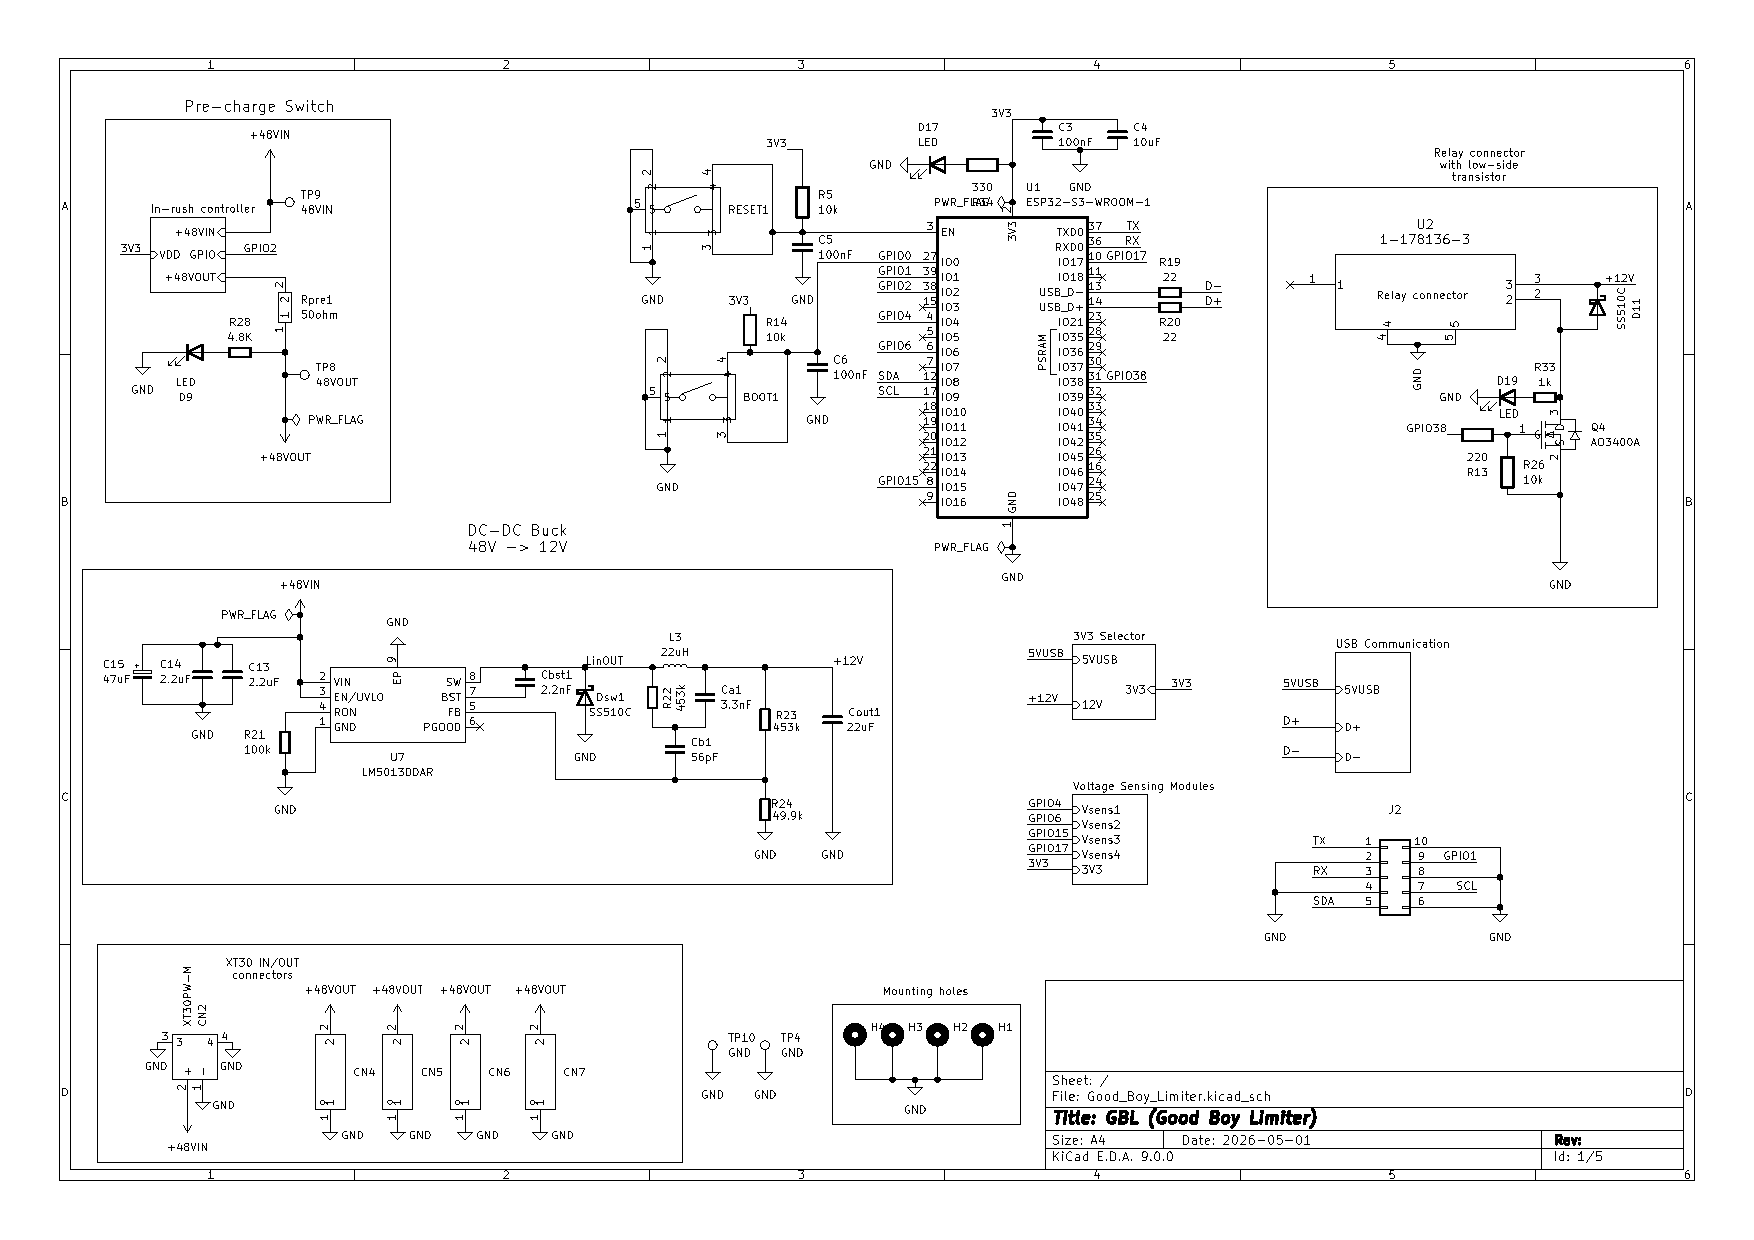
\includegraphics[page=1, width=0.85\textwidth]{Images/Good_Boy_Limiter.pdf}
\end{center}

\includepdf[pages=2-, nup=1x2, scale=0.65, pagecommand={\thispagestyle{plain}}]{Images/Good_Boy_limiter.pdf}


\section{References}
\label{sec:ref}

\begin{itemize}
    \item \href{https://www.ti.com/lit/ds/symlink/lm5069.pdf}{Texas Instruments LM5069 Datasheet}
    \item \href{https://www.ti.com/lit/ds/symlink/lm5013.pdf}{Texas Instrument LM5013DDAR Datasheet}
    \item \href{https://file.elecfans.com/web2/M00/24/31/poYBAGGwZlOAfiG4AAkVY6pkKgU639.pdf?STB15810_ST.pdf}{STMicroelectronics STB15810 Datasheet}
    \item \href{https://mm.digikey.com/Volume0/opasdata/d220001/medias/docus/6778/5399_SY8120B%20SOT-23-6.PDF}{Slkor SY8120B Datasheet}
\end{itemize}

\end{document}